\documentclass[twoside]{article}

\usepackage{amsmath,amsthm,amssymb,graphicx}
\usepackage{hyperref}
\usepackage[numbers]{natbib}
\usepackage{float}
\usepackage{bbm}

\theoremstyle{definition}
\newtheorem{thm}{Theorem}[section]
\newtheorem{lem}[thm]{Lemma}
\newtheorem{prop}[thm]{Proposition}
\newtheorem{cor}[thm]{Corollary}
\newenvironment{pf}{{\noindent\sc Proof. }}{\qed}
\newenvironment{map}{\[\begin{array}{cccc}} {\end{array}\]}

\newcommand{\comment}[1]{}
\theoremstyle{definition}
\newtheorem*{defn}{Definition}
\newtheorem*{exmp}{Example}
\newtheorem*{prob}{Problem}

\theoremstyle{remark}
\newtheorem*{rem}{Remark}
\newtheorem*{note}{Note}
\newtheorem*{exer}{Exercise}

\setlength{\oddsidemargin}{0.25 in}
\setlength{\evensidemargin}{-0.25 in}
\setlength{\topmargin}{-0.6 in}
\setlength{\textwidth}{6.5 in}
\setlength{\textheight}{8.5 in}
\setlength{\headsep}{0.75 in}
\setlength{\parindent}{0 in}
\setlength{\parskip}{0.1 in}

\newcommand{\widgraph}[2]{\includegraphics[keepaspectratio,width=#1]{#2}}
\newcommand{\widgraphr}[3]{\includegraphics[keepaspectratio,width=#1,angle=#3]{#2}}

\newcommand{\lecture}[4]{
   \pagestyle{myheadings}
   \thispagestyle{plain}
   \newpage
   \setcounter{page}{1}
   \noindent
   \begin{center}
   \framebox{
      \vbox{\vspace{2mm}
    \hbox to 6.28in { {\bf Stat365/665 (Spring 2015) Data Mining and Machine Learning \hfill Lecture: #4} }
       \vspace{6mm}
       \hbox to 6.28in { {\Large \hfill #1  \hfill} }
       \vspace{6mm}
       \hbox to 6.28in { {\it Lecturer: #2 \hfill Scribe: #3} }
      \vspace{2mm}}
   }
   \end{center}
   \markboth{#1}{#1}
   \vspace*{4mm}
}


%%%%%%%
% Some commonly used notation
%%%%%%%

\def\R{{\mathbb R}}
\def\X{{\mathcal X}}
\def\Y{{\mathcal Y}}
\def\H{{\mathcal H}}
\def\E{{\mathbb E}}
\def\sign{{\rm sign}}

\newcommand{\percent}{$\%$}

\begin{document}
\textbf{Computer Vision, Homework 4}\\
\textbf{Leon Lixing Yu}\\


\section{Parametrizing Curves}

\subsection{Find $\alpha(s)$}
\[\alpha (s) = (\frac{1}{k} cos(s), \frac{1}{k} sin(s))\]
\[ s \in [-\pi, \pi]\]
\[\alpha'(s) = (-\frac{1}{k} sin(s), \frac{1}{k} cos(s))\]
\[\| \alpha'(s)\| = \sqrt{sin^2(s)+cos^2(s)} = \frac{1}{k}\]

\subsection{Find Frenet approximation to the circle}
\[\alpha''(s) = (-\frac{1}{k} cos(s), -\frac{1}{k} sin(s))\]
\[\alpha (s_0 + s) = \alpha (s_0) + s ( \alpha' (s_0)) + \frac{s^2}{2} \alpha''(s_0)\]
From here we can sub in $\alpha$, $\alpha'$, and $\alpha''$.\\

\subsection{Plot magnitude error}
Before plotting the magnitude, I wants to plot the scatter graph to get a better scene of what's going on, see figure below. 

\begin{figure}[H]
\centering
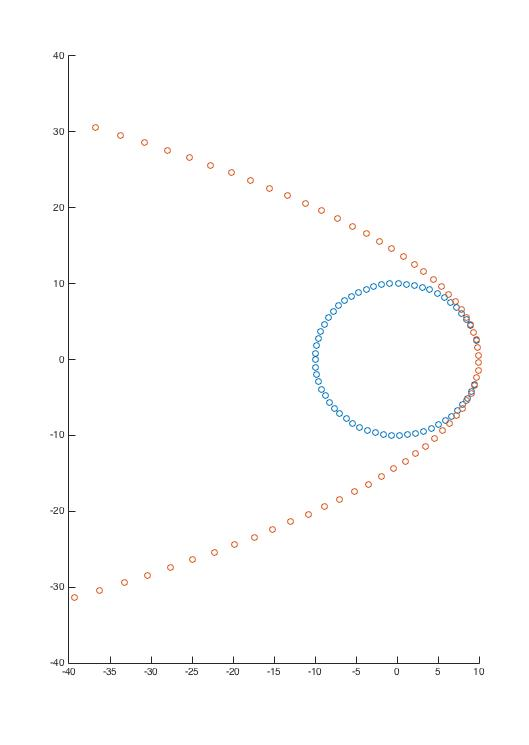
\includegraphics[width=120mm]{scatter.jpg}
\caption{The blue circle is our scatter of $\alpha(s)$, and the red parabola is our scatter of frenet approximation. $s \in [-\pi, \pi]$ In the picture shown, the parabola lies in the plane through $\alpha(s_0)$ orthogonal to $\alpha(s_0)$}
\end{figure}

\begin{figure}[H]
\centering
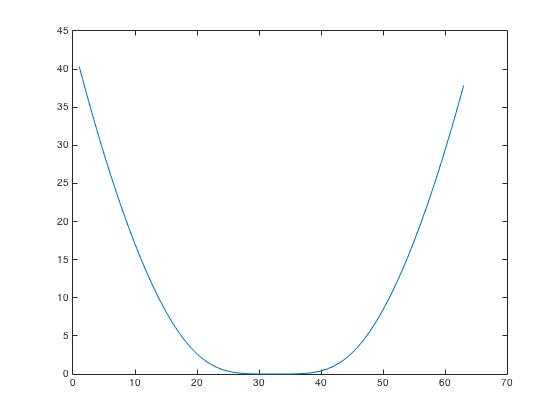
\includegraphics[width=120mm]{01.jpg}
\caption{The x-axis is the number of data points, and y-axis is the magnitude of error, we see that the peak error is around 40 when curvature is 0.1, meaning radius is 10}
\end{figure}

\begin{figure}[H]
\centering
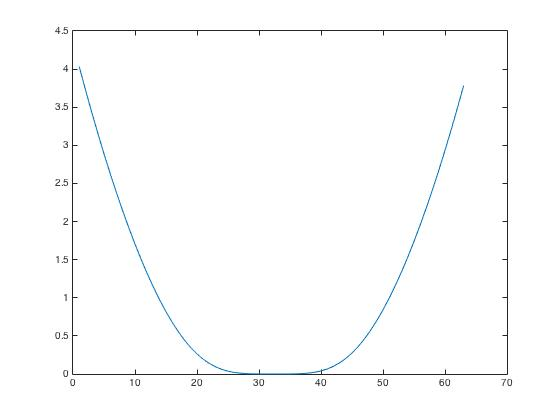
\includegraphics[width=120mm]{1.jpg}
\caption{The x-axis is the number of data points, and y-axis is the magnitude of error, we see that the peak error is around 4 when curvature is 1, meaning radius is 1}
\end{figure}

\begin{figure}[H]
\centering
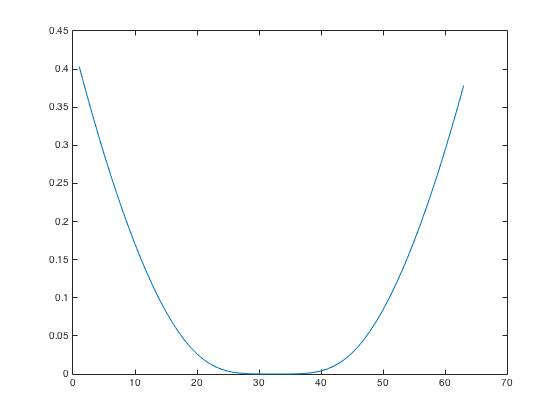
\includegraphics[width=120mm]{10.jpg}
\caption{The x-axis is the number of data points, and y-axis is the magnitude of error, we see that the peak error is around 0.4 when curvature is 10, meaning radius is 0.1}
\end{figure}

The results show that the error is inverse-proportional to the curvature. However, I think the magnitude does not change the fact that the frenet approximation is the best quadratic approximation to $\alpha$ at $s_0$.

\section{Geometric Insights into Shape from Texture}
\subsection{calculate $F_{*p}$}
We have:
\[F_{*p} (\pmb{v}) = \frac{d}{du} (F(\alpha(u))), u=0\]

Given:
\[F(\pmb{p}) = r(\pmb{p}) \pmb{p}\]
\[\Rightarrow \frac{d}{du} (F(\alpha(u))) = \frac{d}{du} (r(\alpha(u)) \alpha(u))
\]
\[=r'((\alpha(u))\alpha(u)+r(\alpha(u))\alpha'(u)\]
We also know that:
\[\alpha(u) = \pmb{p}, \alpha'(u) = \pmb{v}, u = 0\]
Therefore, we have:
\[\Rightarrow F_{*p} (\pmb{v}) = \nabla r \;\pmb{ p} + r \;\pmb{v}\]

\subsection{Prove argmax}
If $\pmb{v} = \nabla r / \| \nabla r \|$, we know that $\pmb{v} $ is tangential to $r$, so the angle between $r$ and $\pmb{v} $ is 0. Plug it back to the equation above:
\[\| F_{*p} (\pmb{v}) \| =\| \nabla r \;\pmb{ p} + r ( \nabla r / \| \nabla r \|) cos(0) \|\]
This form will clearly reach optima as $cos(0)$ equal to 1. 

If $v$ is tangential to $r$, we can just move $v$ from viewsphere at $p$ to our surface $s$.  

\subsection{Show $F_*(t)$ is orthogonal to $F_*(b)$}




\end{document}
